\subsection{Bucketsort}
\label{section:bucketsort}

Der \currentauthor{Florian Grieskamp} Bucketsort-Algorithmus \cite[Kapitel 8.2 (dort unter dem Namen \emph{counting sort})]{Cormen2009} ist ein Sortierverfahren, das für Werteverteilungen über einem Alphabet einer konstanten Größe Eingaben in linearer Zeit sortieren kann. Da die Bedingung einer konstanten Alphabetgröße allerdings häufig nicht erfüllt ist, wird Bucketsort oft in Verbindung mit einer Schlüsselfunktion verwendet, um gemäß des Schlüssels \glqq ähnliche\grqq{} Werte zu gruppieren. Diese gruppierten Bereiche werden als \emph{Buckets} bezeichnet und im Anschluss mit einem anderen Sortierverfahren verfeinert. Bucketsort dient in dieser Variante als Mechanismus zur groben Vorsortierung.\par
\begin{definition}[Bucket]
	\label{def:bucket}
	Ein Intervall \(\bucket{} \coloneqq \sa[l, r]\) des Suffixarrays begrenzt durch einen linken Index \(l\) und einen rechten Index \(r\) heißt Bucket.\par
    Falls alle in einem Bucket \(\bucket{p} \coloneqq \sa[l, r]\) enthaltenen Suffixe, also die Suffixe \(\suffix{\sa[l]}, \suffix{\sa[l+1]}, \ldots, \suffix{\sa[r]}\), einen gemeinsamen Präfix \(p\) der Länge \(m\) haben, so heißt \(\bucket{p}\) Level-\(m\)-Bucket.
\end{definition}
Da im Anwendungsfeld der Suffixarray-Konstruktion die zu sortierenden Elemente Suffixe über \(\Sigma^\ast\) sind, ist eine Schlüsselfunktion notwendig, die Wertebereich einschränkt. Hier werden als Schlüssel gemeinsame Präfixe der Länge \(d\) (für Bucketsort mit Tiefe \(d\)) verwendet.\par
Der Algorithmus besteht aus drei iterativ durchgeführten Schritten, die hier erläutert werden. Als begleitendes Beispiel dient die Sortierung der Suffixe des Wortes \emph{caabaccaabacaa} mit der Tiefe 2.
\paragraph{Schritt 1}
Es wird zunächst ein Hilfsarray (\cref{bucketsort:bkt}) angelegt, in dem zu jedem möglichen Schlüssel (hier Präfixe über \(\Sigma^2\)) dessen Häufigkeit in der Eingabe vermerkt wird. Dies geschieht anhand eines sequentiellen Scans der Eingabesequenz. Diese Anzahl legt die Größe des jeweiligen Buckets fest. In einem Scan des Hilfsarrays kann dann In-Place die kumulative Summe der Größen bestimmt werden, durch welche die Grenzen zwischen den Buckets festgelegt werden.
\begin{figure}[ht]
    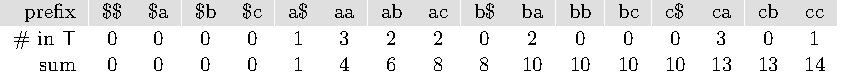
\includegraphics[width=\textwidth]{kapitel/4_komponenten/sortieralgorithmen/bucketsort/step_01/bkt/image.pdf}
    \caption{Bestimmung der Bucketgrößen und Startpositionen}
    \label{bucketsort:bkt}
\end{figure}
\paragraph{Schritt 2}
Um die Elemente sortieren zu können, wird ein zweites Array in der Länge der Eingabesequenz angelegt. Dieses Array ist auf Basis der zuvor berechneten Grenzen (imaginär) in Buckets eingeteilt (\cref{bucketsort:empty_buckets}).
\begin{figure}[ht]
    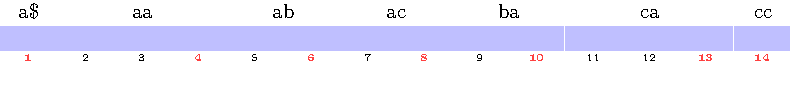
\includegraphics[width=\textwidth]{kapitel/4_komponenten/sortieralgorithmen/bucketsort/step_02/empty_buckets/image.pdf}
    \caption{Buckets ohne einsortierte Suffixe}
    \label{bucketsort:empty_buckets}
\end{figure}
In einem Scan der Eingabesequenz wird dann iterativ für jedes Element der zugehörige Schlüssel berechnet, um anhand der Tabelle aus \cref{bucketsort:bkt} die Position im Ausgabearray zu bestimmen. Nach dem Einfügen an dieser Position wird die Grenze des jeweiligen Buckets entsprechend angepasst, um bereits eingefügte Elemente im Nachhinein nicht mit neuen Elementen zu überschreiben.\par
Nach Abschluss dieses Schritts liegen die vorsortierten Elemente der Eingabesequenz in korrekter Reihenfolge bezüglich des gewählten Sortierschlüssels im Ausgabearray (\cref{bucketsort:buckets}).
\begin{figure}[ht]
    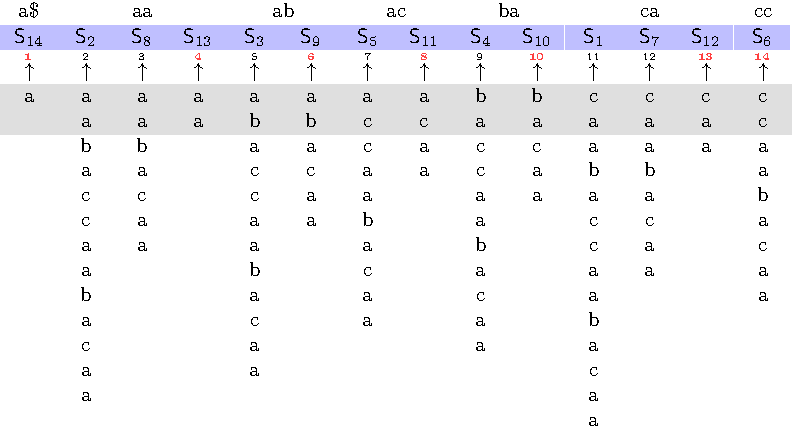
\includegraphics[width=\textwidth]{kapitel/4_komponenten/sortieralgorithmen/bucketsort/step_02/buckets/image.pdf}
    \caption{Buckets mit einsortierten Suffixen}
    \label{bucketsort:buckets}
\end{figure}
\paragraph{Schritt 3 (optional)}
Je nach Anwendungsfall kann es erwünscht sein, dass die Elemente in sortierter Reihenfolge direkt im Eingabearray liegen. Falls dies erforderlich ist, so wird in einem dritten Scan der Inhalt des Ausgabearrays ins Eingabearray kopiert und dabei die alte Eingabe überschrieben. Die Weiterverarbeitung der einzelnen Buckets erfolgt dann mit einem anderen Sortieralgorithmus oder wahlweise auch weiter mit Bucketsort unter Verwendung einer anderen Schlüsselfunktion.
